\documentclass[xcolor=table]{beamer}
\usepackage[table,xcdraw]{xcolor}
\usepackage[utf8]{inputenc}
\usepackage{epigraph}
\usepackage{graphicx}
\usepackage[left=25mm,right=25mm,top=2cm,bottom=2cm]{geometry}
\usepackage{indentfirst}
\usepackage{hyperref}
\usepackage{amsmath}
\usepackage{xcolor}
\usepackage{float}
\usepackage{wrapfig}
\usepackage{subfig}
\usepackage{derivative}
\usepackage[table,xcdraw]{xcolor}
\usepackage[english, russian]{babel}
\usepackage{setspace}
\usepackage{hyperref}

\usetheme{Madrid}
\usecolortheme{spruce}

%------------------------------------------------------------
%This block of code defines the information to appear in the
%Title page
\title[Хакатон МФТИ 15.11 - 18.11]{Хакатон МФТИ 15.11 - 18.11}

%\subtitle{Начало}

\author[М. Анош, Е. Мас, В. Кар, Н. Косм] 
{М.~Аношин\inst{1} \and Е.~Масов\inst{1} \and В.~Карецкий\inst{1} \and Н.~Космынин\inst{1}}

\date[18.11.2022] 
{МФТИ, Ноябрь 2022}

\begin{document}
\frame{\titlepage}

\section{Часть 1}
\begin{frame}\frametitle{Открытые банки сигналов ЭКГ, репрезентативность выбранных данных}

В нашей работе мы использовали следующие источники

\begin{enumerate} 
    \item \href{https://www.physionet.org/content/ptbdb/1.0.0/}{PTB Diagnostic ECG Database}
    \item \href{https://www.physionet.org/content/mitdb/1.0.0/}{MIT-BIH Arrhythmia Database (использовался для очистки данных от ''лишних'' случаев)}
    \item \href{https://www.physionet.org/content/noneeg/1.0.0/}{Non-EEG Dataset for Assessment of Neurological Status (анализ ECG для определения изменения характеристик в зависимости от состояния человека)}
    
\end{enumerate}

Принципы выбора данных: 
\begin{enumerate} 
    \item Большая выборка участников исследования
    (порядка $300$ человек)
    \item Однородность базы по состоянию здоровья участников 
    (либо все здоровы, либо больные распределены ''равномерно'')
    \item Частота дискретизации прибора ЭКГ(для объективного сопоставления полученных результатов)
\end{enumerate}

\end{frame}


\section{Часть 2}
\begin{frame}{Обработка измерений}
    %Красивые картиночки в стиле было/стало
    %Можно выделить пики желтыми кружками
Чтение данных 
\begin{enumerate}
    \item $*.dat *.art *.hea$
    
    Чтение волновых осциллограмм
    
    \item $*.edf$

\end{enumerate}

Нормализация данных
\begin{enumerate}
    \item $min\_max\_scaller$

    Нормализация данных по среднему и нормиповка по максиуму
    
    \item $standart\_scaller$

    Классическая нормализация данных
    
\end{enumerate}

Алогритмы/Классификации
\begin{enumerate}
    \item $Moving Average$
    
    И другие фильтры оцифровки сигналов, для обработки RR/NN пиков
    
    \item $Fast-Fourier Transform$

    Классический алгоритм для разбиения сигнала на гармоники
    
\end{enumerate}


\end{frame}

\begin{frame}{Анализ данных}
\centering
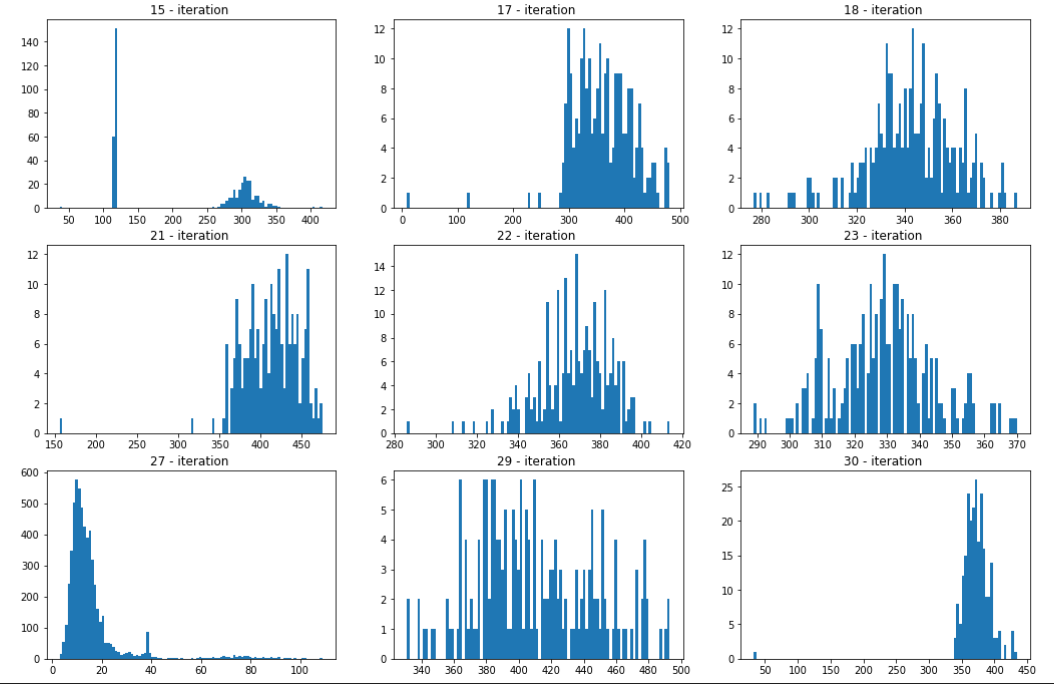
\includegraphics[height=7cm]{Распределение3.png}
\end{frame}

\begin{frame}{Гистаграммы, построенные на основе анализа данных}
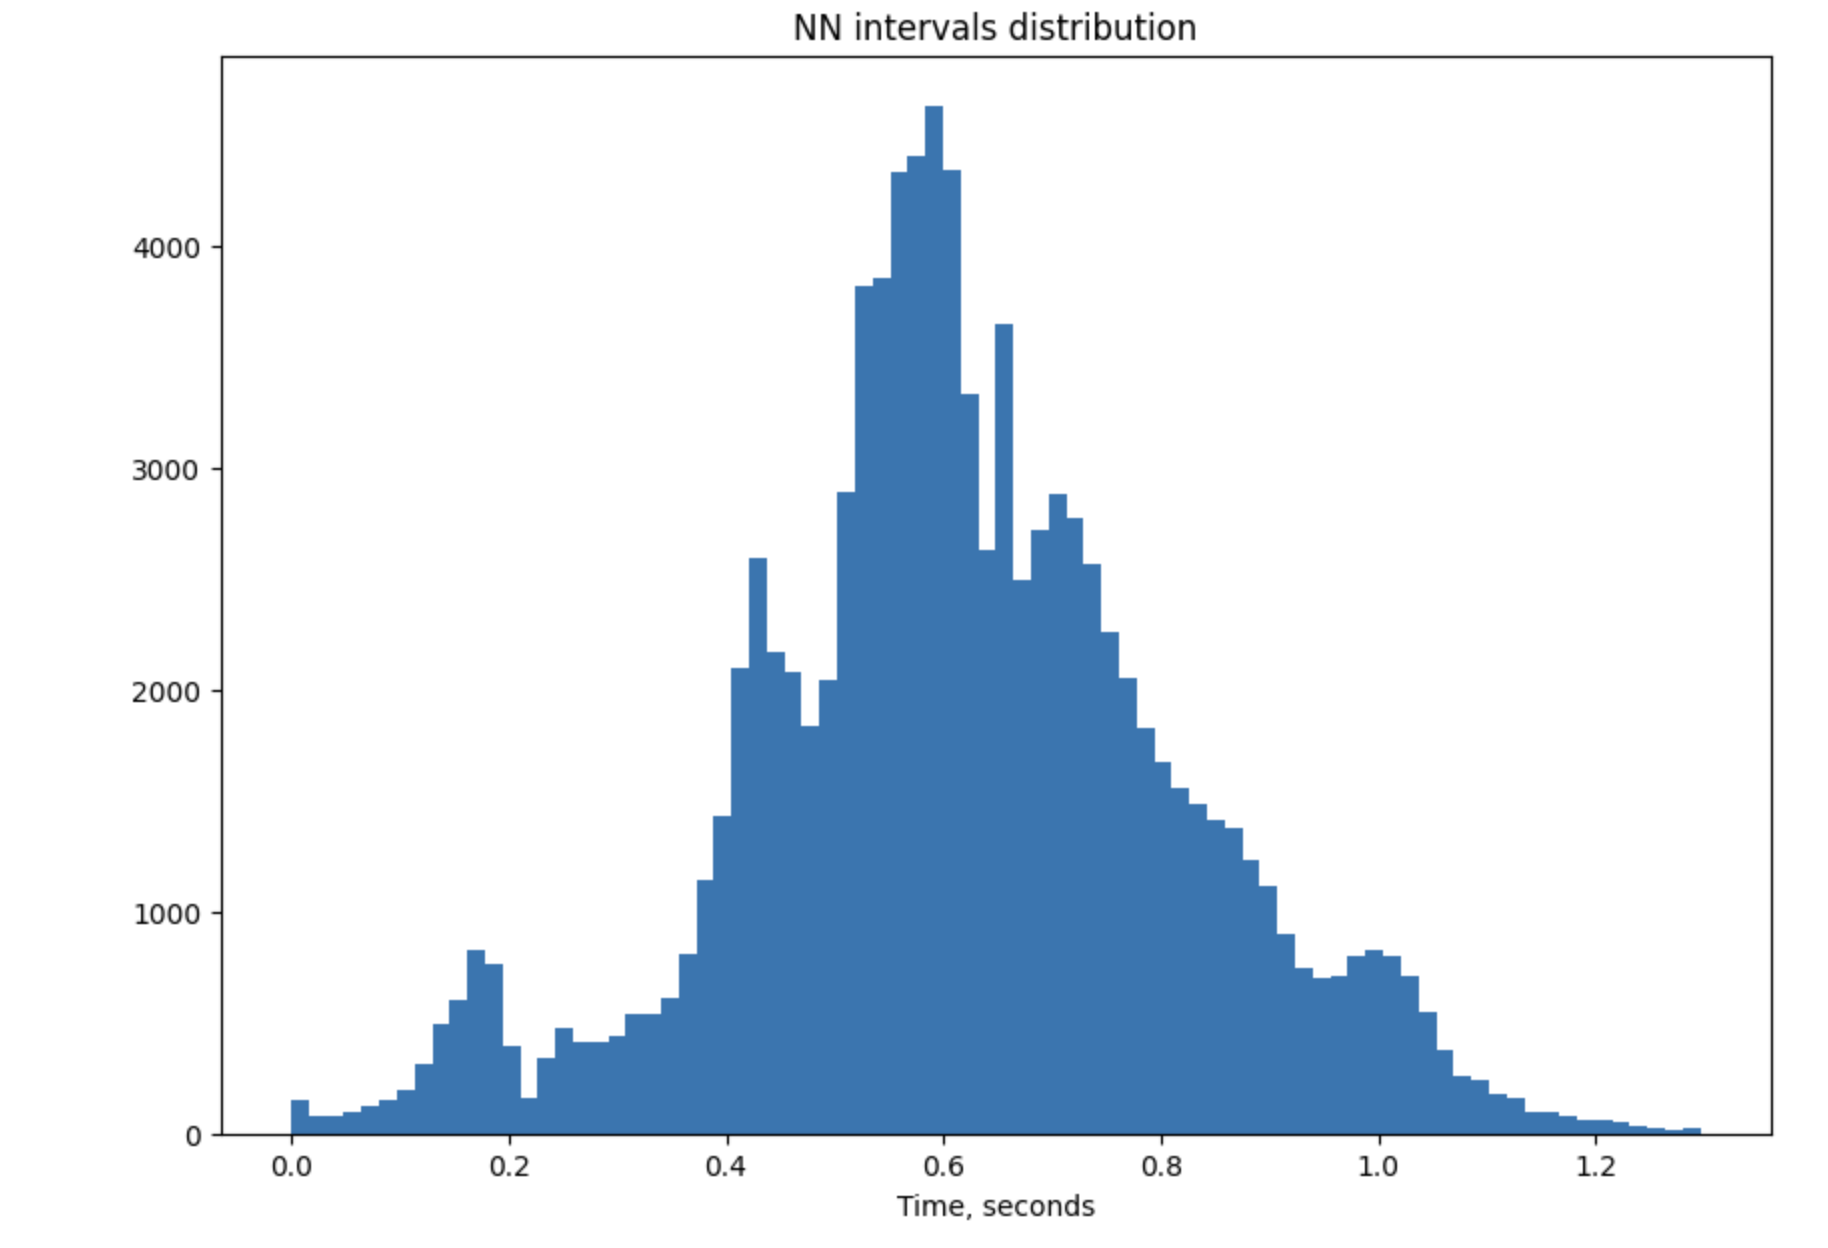
\includegraphics[height=3.8cm]{Распределение1.png}
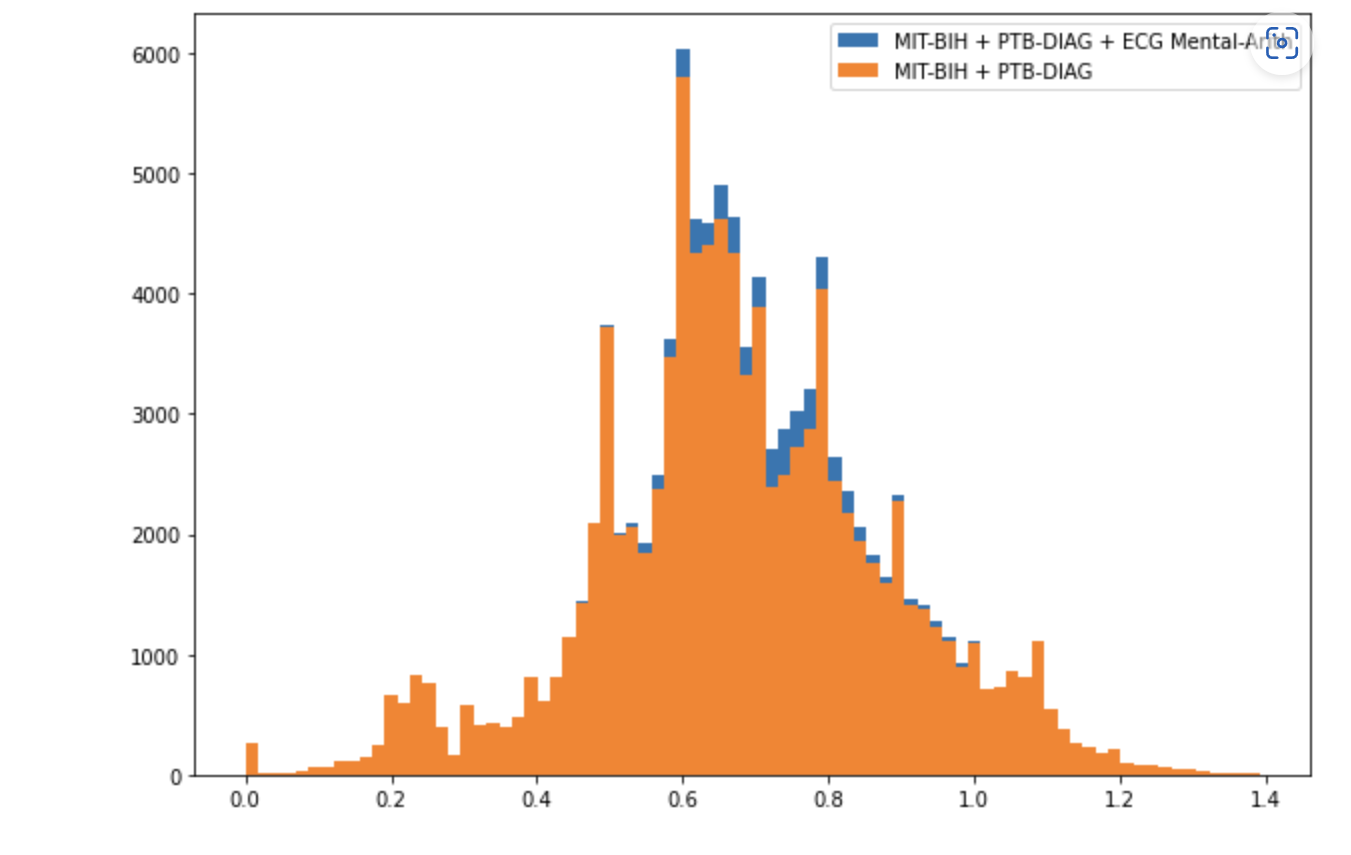
\includegraphics[height=3.8cm]{Распределение2.png}
\end{frame}




\section{Часть 3}
\begin{frame}{Расчет параметров статистического анализа хронокардиограмм}

\centering
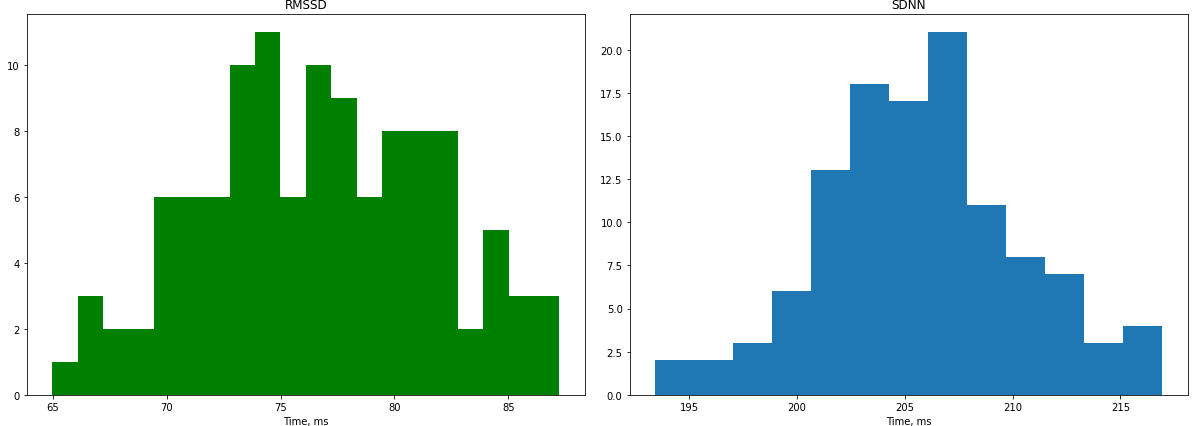
\includegraphics[height=4.2cm]{graph2.png}

\end{frame}


\begin{frame}{Расчет параметров статистического анализа хронокардиограмм}
\centering
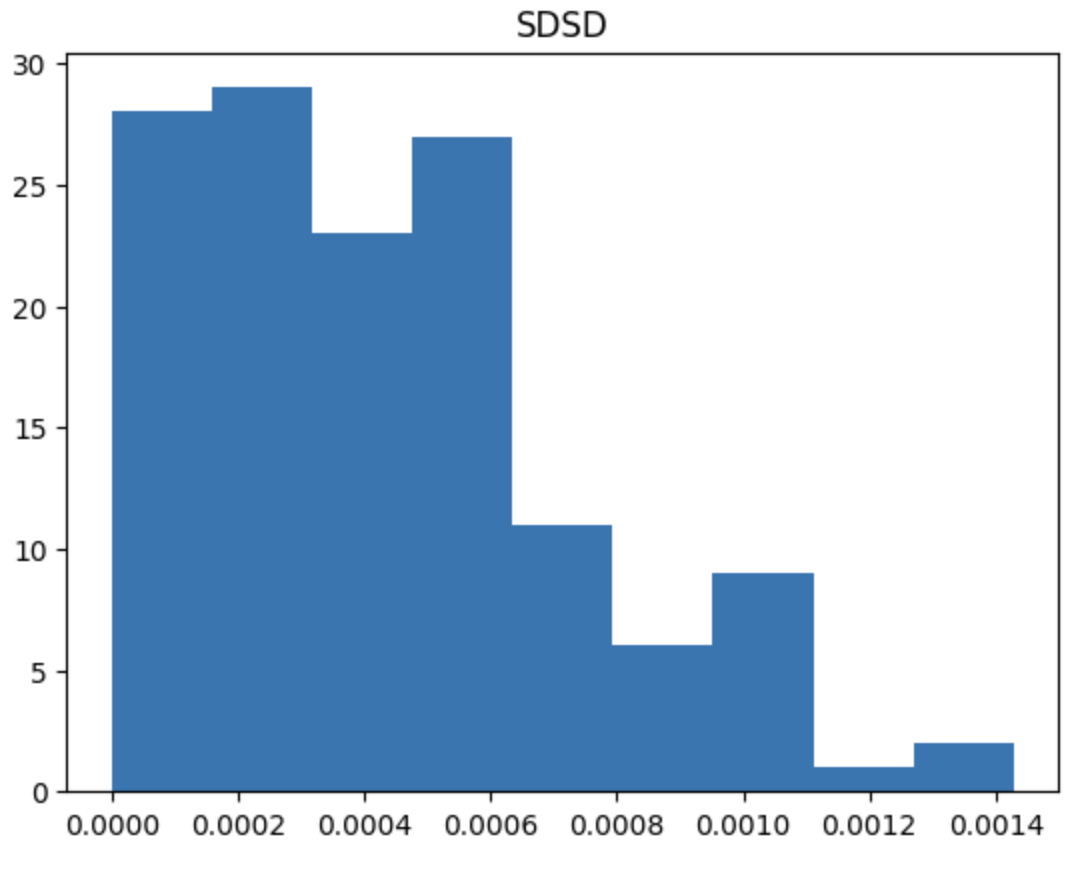
\includegraphics[height=6cm]{SDSD.png}

\end{frame}

\begin{frame}{Расчет параметров статистического анализа хронокардиограмм}
    \centering
    \Large
    $$pNN50 = 0.29$$
    $$pNN20 = 0.21$$
\end{frame}


\begin{frame}{Интепретация результатов}
\centering
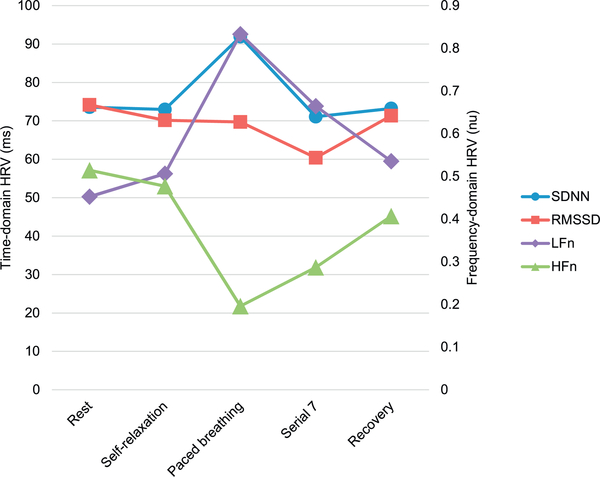
\includegraphics[height=7cm]{images/nihms-1022910-f0001.jpg}
\vspace{5}

\small \href{https://www.ncbi.nlm.nih.gov/pmc/articles/PMC6492031/}{[2018 Nov 8. doi: 10.1016/j.physbeh.2018.11.009]}
\end{frame}


\begin{frame}{Дальнейшее развитие в области}
\begin{enumerate} 
    \item \href{https://www.ncbi.nlm.nih.gov/pmc/articles/PMC8348698/}{[2021 Jul 23. doi: 10.3390/s21155015] Статья обращает внимание на существующие датасеты с EEG и ECG полученные, например, путем анализа сигналов людей, смотрящих видео разной эмоциональной окраски}
    \item \href{https://iopscience.iop.org/article/10.3847/1538-4365/aab766}{[Jacob T. VanderPlas 2018 ApJS 236 16, doi: 10.3847/1538-4365/aab766] Применение методики Ломба-Скаргла, для поиска не явных повторяющихся гармоник в ECG (вместо FFT)}
\end{enumerate}
    
\end{frame}


\begin{frame}{Необходимые ресуры для практического приложения}
\begin{enumerate}
    \item \href{https://www.intechopen.com/chapters/53607}{Использовние полупроводниковых элементов, таких, как
    мемристр, для аппаратного поиска пиков и разложение в ряд Фурье}
\end{enumerate}
\centering
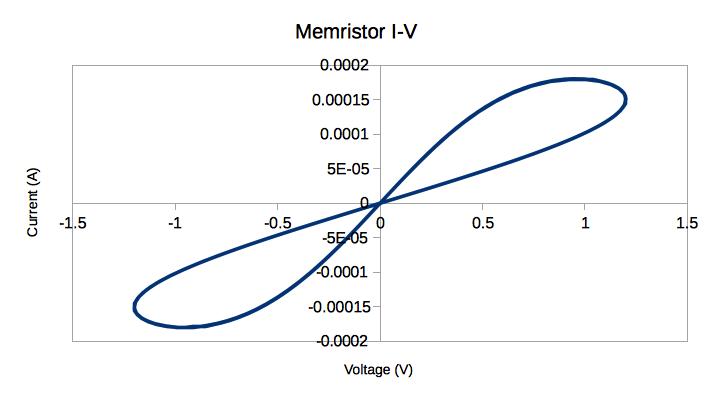
\includegraphics[height=4cm]{MemristorI-V.png}
\end{frame}



\end{document}